
\let\negthickspace\undefined
\documentclass[journal]{IEEEtran}
\usepackage[a5paper, margin=10mm, onecolumn]{geometry}
%\usepackage{lmodern} % Ensure lmodern is loaded for pdflatex
\usepackage{tfrupee} % Include tfrupee package

\setlength{\headheight}{1cm} % Set the height of the header box
\setlength{\headsep}{0mm}     % Set the distance between the header box and the top of the text

\usepackage{gvv-book}
\usepackage{gvv}
\usepackage{cite}
\usepackage{amsmath,amssymb,amsfonts,amsthm}
\usepackage{algorithmic}
\usepackage{graphicx}
\usepackage{textcomp}
\usepackage{xcolor}
\usepackage{txfonts}
\usepackage{listings}
\usepackage{enumitem}
\usepackage{mathtools}
\usepackage{gensymb}
\usepackage{comment}
\usepackage[breaklinks=true]{hyperref}
\usepackage{tkz-euclide} 
\usepackage{listings}
% \usepackage{gvv}                                        
\def\inputGnumericTable{}                                 
\usepackage[latin1]{inputenc}                                
\usepackage{color}                                            
\usepackage{array}                                            
\usepackage{longtable}                                       
\usepackage{calc}                                             
\usepackage{multirow}                                         
\usepackage{hhline}                                           
\usepackage{ifthen}                                           
\usepackage{lscape}
\begin{document}

\bibliographystyle{IEEEtran}
\vspace{3cm}

\title{9.2.12}
\author{EE24BTECH11053 - S A Aravind Eswar}
% \maketitle
% \newpage
% \bigskip
{\let\newpage\relax\maketitle}

\renewcommand{\thefigure}{\theenumi}
\renewcommand{\thetable}{\theenumi}
\setlength{\intextsep}{10pt} % Space between text and floats


\numberwithin{equation}{enumi}
\numberwithin{figure}{enumi}
\renewcommand{\thetable}{\theenumi}

\textbf{Question: } Find the area of region bounded by the curse $x^2 = 4y$,  $y=2$, $y=4$ and the y-axis in the first quadrant. 

\solution
\begin{table}[h]
    \centering
    \begin{tabular}{|m{5em} | m{7em} | m{10em} |}
    \hline
    \textbf{symbol} & \textbf{Value} & \textbf{Description}\\
    \hline
        \textbf{V},\textbf{u},f & $\myvec{ 1 & 0\\0 & 0}$, $\myvec{0\\2}$, 0 & Parameters of the given conic (parabola)\\
    \hline
        $\vec{h_1}, \vec{m_1}$ & $\myvec{0\\2}, \myvec{1\\0}$ & Parameters of the given line $y = 2$\\
    \hline
        $\vec{h_2}, \vec{m_2}$ & $\myvec{0\\4}, \myvec{1\\0}$ & Parameters of the given line $y = 4$\\
    \hline
        $\vec{a_1}, \vec{a_2}$ & & Points of intersection of given lines to the conic\\
    \hline
        $\kappa_i$ & & Parameters of the line equation $\vec{x} = \vec{h} + \kappa\vec{m}$\\
    \hline
        $A_1$ & & Area under the parabola from $y=0$ to $y=4$\\
    \hline
        $A_2$ & & Area under the parabola from $y=0$ to $y=2$\\
    \hline
\end{tabular}

    \caption{Given Values}
    \label{tab:1}
\end{table}

Using,
\begin{align}
    \kappa_i = \frac{1}{\vec{m}^\top\vec{V}\vec{m}}\brak{-\vec{m}^\top\brak{\vec{Vh}+\brak{u}}\pm \sqrt{\sbrak{\vec{m}^\top\brak{\vec{Vh}+\vec{u}}}^2 - g(\vec{h})(\vec{m}^\top\vec{Vm})}}
\end{align}
and substituting in the line equation,
\begin{align}
    \vec{x} = \vec{h} + \kappa\vec{m}
\end{align}
we can find the points of intersection of the given lines and the conic in the first quadrant to be,
\begin{align}
    \vec{a_1} = \myvec{2\sqrt{2}\\2}, \vec{a_2} = \myvec{4\\4}
\end{align}
Calculating $A_1 \text{ and } A_2$,
\begin{align}
    A_1 = \int_{0}^{4} \frac{x^2}{4} dx = \frac{16}{3}\\
    A_2 = \int_{0}^{2\sqrt{2}} \frac{x^2}{4} dx = \frac{4\sqrt{2}}{3}
\end{align}
Thus, the area of the parabola between the lines $y = 2$ and $y = 4$ is,
\begin{align}
    (\int_{0}^{4} 4 dx - A_1) - (\int_{0}^{2\sqrt{2}} 2 dx - A_2) = \frac{32 - 8\sqrt{2}}{3}
\end{align}

\begin{figure}[h]
    \centering
    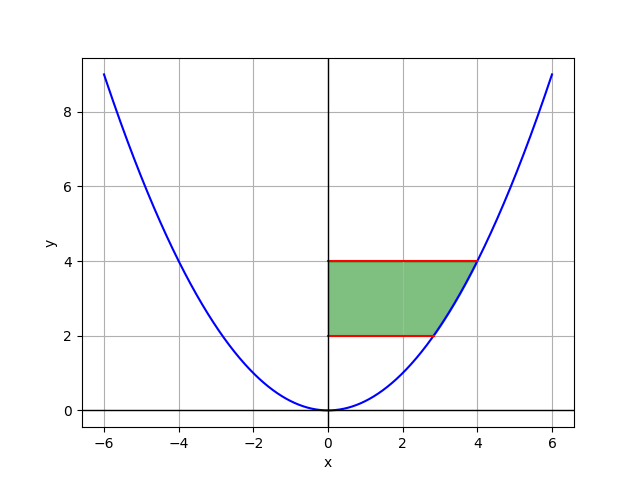
\includegraphics[width=\columnwidth]{figs/fig1.png}
    \caption{Area Under the graph}
\end{figure}

\end{document}  

